\labeledsection{Regression}{sec:regression}
\anondefinition{
A \linkterm{function}{function} with one argument is called \defemph{univariate} or \defemph{unary}
}{univariate}

\anondefinition{
A \linkterm{univariate}{univariate} function $f : \mathbb{R} \to \mathbb{R}$ is called \defemph{linear} iff it simply scales its input by a constant factor:
\[
f(x) = wx
\]
for some constant scalar $w \in \mathbb{R}$.
}{linear_function_scalar}

\observationbox{
Geometrically, this represents a straight line that passes exactly through the origin $(0,0)$.
}

\Example{
If $w = 3$, then $f(x) = 3x$. 
\begin{itemize}
    \item If $x = 2 \implies f(2) = 6$
    \item If $x = 0 \implies f(0) = 0$
\end{itemize}
}{}
 
\anondefinition{
A \linkterm{univariate}{univariate} function $h_w : \mathbb{R} \to \mathbb{R}$ of the form:
\[
h_w(x) = w_1x + w_0
\]
is called an \defemph{affine linear model}. The parameter $w_1$ is a scalar called the \defemph{slope}, and $w_0$ is a scalar called the \defemph{intercept} or \defemph{bias}.
}{affine_linear_model_scalar}

\observationbox{
An \linkterm{affine linear function}{affine_linear_model_scalar} is simply a \textbf{strict linear} \linkterm{function}{function} plus a constant baseline offset. Because of the $+ w_0$ term, if you pass in zero, the output is the offset ($h_w(0) = w_0$). Geometrically, this is a straight line that can cross the vertical axis anywhere, not just at the origin.
}

\Example{
Let $w_1 = 3$ and $w_0 = 2$, which gives the model $h_w(x) = 3x + 2$.
\begin{itemize}
    \item If $x = 2 \implies h_w(2) = 3(2) + 2 = 8$
    \item If $x = 0 \implies h_w(0) = 3(0) + 2 = 2$
\end{itemize}
}{}

\anondefinition{
Let $E \subseteq \mathbb{R} \times \mathbb{R}$ be a \linkterm{set}{def:set} of \linkterm{examples}{supervised_learning} (where each example is a pair of scalar inputs and scalar outputs $(x_i, y_i)$). The task of finding the constant scalars $w_1$ and $w_0$ such that the \linkterm{affine linear model}{affine_linear_model_scalar} $h_w(x) = w_1x + w_0$ fits the data points in $E$ as closely as possible is called \defemph{univariate linear regression}.
}{univariate_linear_regression}

\observationbox{
In this task, we are strictly mapping a single scalar input variable to a single scalar output variable. Geometrically, this means finding the optimal straight line through a cloud of data points on a two-dimensional grid.
}

\Example{
We have a dataset $E = \{ (1, 3), (2, 5), (3, 7) \}$. The goal of univariate linear regression is to find the scalars $w_1$ and $w_0$. Here, the perfect fit is reached when $w_1 = 2$ and $w_0 = 1$, yielding the model $h_w(x) = 2x + 1$.
}{}

\questionbox{
How to find parameters $w$?
}

\ideabox{
We minimize \linkterm{$\ell_2$ Loss}{l2_loss}
}

\titledbox{Remember}{
\linkterm{$\ell_2$ Loss}{l2_loss} (squared error loss) for $N$ \linkterm{examples}{supervised_learning} is $\sum_{i=1}^N \big(y_i-\hat{y_i}\big)^2$
}

\solutionbox{
We have to find the best tuple $w$, call it $w^{*}$. 

\[
w^{*} := \argmin{w_0, w_1} \sum_{i=1}^{N} \big(y_i-(w_1x_i + w_0)\big)^2
\]
}

\observationbox{
\[
\sum_{i=1}^{N} \big(y_i-(w_1x_i+w_0)\big)^2
\]
is differentiable, a minimum is attained when its partial derivatives with respect to the parameters vanish ($=0$).
}

Let $L(h_w) = \sum_{i=1}^{N} \big(y_i-(w_1x_i+w_0)\big)^2$. To minimize the loss, we find where the partial derivatives with respect to each parameter vanish ($=0$):
\[
\frac{\partial L}{\partial w_0}=0
\qquad
\text{and}
\qquad
\frac{\partial L}{\partial w_1}=0
\]

Applying the chain rule ($\frac{d}{dx}[g(x)^2] = 2g(x) \cdot g'(x)$), the derivatives distribute inside the summation:
\[
\frac{\partial L}{\partial w_0} = \sum_{i=1}^{N} 2\big(y_i-(w_1x_i+w_0)\big)(-1)
\]
\[
\frac{\partial L}{\partial w_1} = \sum_{i=1}^{N} 2\big(y_i-(w_1x_i+w_0)\big)(-x_i)
\]

Setting these total gradients to zero yields the normal system of equations:
\begin{equation}
\sum_{i=1}^{N} 2\big(y_i-(w_1x_i+w_0)\big)(-1) = 0 \label{eq:w0}
\end{equation}
\begin{equation}
\sum_{i=1}^{N} 2\big(y_i-(w_1x_i+w_0)\big)(-x_i) = 0 \label{eq:w1}
\end{equation}

Solving for $w_0$
Divide equation \eqref{eq:w0} by $-2$ and expand the summation across the individual scalar terms:
\[
\sum_{i=1}^{N} \big(y_i - w_1x_i - w_0\big) = 0
\]
\[
\sum_{i=1}^{N} y_i - w_1\sum_{i=1}^{N} x_i - \sum_{i=1}^{N} w_0 = 0
\]

Because $w_0$ is a constant independent of the index $i$, summing it $N$ times simplifies to $\sum_{i=1}^{N} w_0 = N w_0$:
\[
\sum_{i=1}^{N} y_i - w_1\sum_{i=1}^{N} x_i - N w_0 = 0
\]

Isolating $N w_0$ gives the explicit baseline offset formula:
\begin{equation}
w_0 = \frac{\sum_{i=1}^{N}y_i - w_1 \sum_{i=1}^{N}x_i}{N} \label{eq:w0_solved}
\end{equation}

Solving for $w_1$
Divide equation \eqref{eq:w1} by $-2$ and distribute the factor of $x_i$ inside the parenthesis:
\[
\sum_{i=1}^{N} \big(y_i - w_1x_i - w_0\big)x_i = 0
\]
\[
\sum_{i=1}^{N} x_i y_i - w_1\sum_{i=1}^{N} x_i^2 - w_0\sum_{i=1}^{N} x_i = 0
\]

Substitute our expression for $w_0$ from equation \eqref{eq:w0_solved} into this expression:
\[
\sum_{i=1}^{N} x_i y_i - w_1\sum_{i=1}^{N} x_i^2 - \left(\frac{\sum_{i=1}^{N}y_i - w_1 \sum_{i=1}^{N}x_i}{N}\right)\sum_{i=1}^{N} x_i = 0
\]

Multiply the entire equation by $N$ to clear out the denominator:
\[
N\sum_{i=1}^{N} x_i y_i - N w_1\sum_{i=1}^{N} x_i^2 - \left(\sum_{i=1}^{N}y_i\right)\left(\sum_{i=1}^{N} x_i\right) + w_1\left(\sum_{i=1}^{N}x_i\right)^2 = 0
\]

Group all terms containing $w_1$ on one side of the equation:
\[
w_1 \left[ N\sum_{i=1}^{N} x_i^2 - \left(\sum_{i=1}^{N}x_i\right)^2 \right] = N\sum_{i=1}^{N} x_i y_i - \left(\sum_{i=1}^{N}x_i\right)\left(\sum_{i=1}^{N}y_i\right)
\]


\observationbox{
The equations \eqref{eq:w0} and \eqref{eq:w1} yield a unique closed-form solution:
}

\[
w_1 = \frac{N(\sum_{i=1}^{N} x_i y_i) - (\sum_{i=1}^{N}x_i) (\sum_{i=1}^{N}y_i)}
{N(\sum_{i=1}^{N}x_i^2) - (\sum_{i=1}^{N}x_i)^2}
\qquad
w_0 = \frac{(\sum_{i=1}^{N}y_i) - w_1 (\sum_{i=1}^{N}x_i)}{N}
\]

\observationbox{
Thus, \linkterm{univariate linear regression}{univariate_linear_regression} admits an exact closed-form solution and does not require iterative optimization methods.
}

\anondefinition{
The \defemph{weight space} of a parametric model is the space of all possible combinations of the parameters (weights). Loss minimization in a weight space is called \defemph{weight fitting}
}{weight_space}

\observationbox{
The \linkterm{weight space}{weight_space} of \linkterm{univariate linear regression}{univariate_linear_regression} is $\mathbb{R}^2$
}

\commandnote{
The \linkterm{$\ell_2$ Loss}{l2_loss} is \textbf{convex} for any \linkterm{univariate linear regression}{univariate_linear_regression} problem $\leadsto$ there are no \textit{local minima}

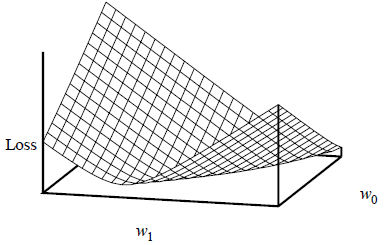
\includegraphics[width=0.3\linewidth]{images/convex.png}
}

\anondefinition{
A \linkterm{function}{function} that takes a collection of $n \geq 2$ distinct input arguments $(x_1, x_2, \dots, x_n)$ and maps them to a single scalar output is called \defemph{multivariate}.
}{multivariate}

\observationbox{
Following the same logic as the \linkterm{univariate}{univariate} \linkterm{affine function}{affine_linear_model_scalar}, a \textbf{multivariate affine function} scales each individual input argument by its own distinct scalar weight ($w_i$) and adds a shared baseline intercept ($w_0$):
\[
f(x_1, \dots, x_n) = w_0 + w_1x_1 + w_2x_2 + \dots + w_nx_n = w_0 + \sum_{i=1}^{n}w_ix_i
\]
where all parameters $w_0, w_1, \dots, w_n$ are individual scalars.
}

\anondefinition{
Let $E \subseteq \mathbb{R}^n \times \mathbb{R}$ be a \linkterm{set}{def:set} of \linkterm{examples}{supervised_learning} (where each example consists of $n$ scalar inputs and one scalar output $(x_{i,1}, x_{i,2}, \dots, x_{i,n}, y_i)$). The task of finding the constant scalar parameters $w_0, w_1, \dots, w_n$ such that the model:
\[
h_w(x_1, \dots, x_n) = w_0 + w_1x_1 + w_2x_2 + \dots + w_nx_n
\]
fits the data points in $E$ as closely as possible is called \defemph{multivariate linear regression}.
}{multivariate_linear_regression}

\observationbox{
Geometrically, instead of fitting a 2D straight line to a flat grid of data points, \linkterm{multivariate linear regression}{multivariate_linear_regression} with $n=2$ features fits a flat 3D plane through a cloud of data points in a three-dimensional space. For $n > 2$, it fits a flat multi-dimensional hyperplane.
}

\notationbox{
To avoid writing out long summations for $n$ features, we package our individual scalar inputs and scalar weights into \textbf{vectors}. 

First, we define a parameter weight vector:
\[
\mathbf{w} :=
\begin{pmatrix}
w_0\\
w_1\\
\vdots\\
w_n
\end{pmatrix}
\]
Next, to account for the baseline intercept $w_0$, we introduce a constant dummy scalar $x_0 := 1$. This allows us to define our complete input feature vector:
\[
\mathbf{x} :=
\begin{pmatrix}
x_0\\
x_1\\
\vdots\\
x_n
\end{pmatrix}
\]

Using these vector representations, the entire multivariate affine model can be compressed compactly into a single matrix multiplication or dot product:
\[
h_{\mathbf{w}}(\mathbf{x})
=
\mathbf{w}^T\mathbf{x}
=
\mathbf{w} \cdot \mathbf{x}
=
\sum_{i=0}^{n} w_i x_i
\]
where $\mathbf{w}^T\mathbf{x}$ denotes matrix multiplication (multiplying a horizontal row vector by a vertical column vector) and $\mathbf{w} \cdot \mathbf{x}$ denotes the standard algebraic dot product.
}

\notationbox{
When we have a dataset of $N$ training examples, we use a superscript $(i)$ to denote the $i$-th example vector. Each individual example vector $\mathbf{x}^{(i)}$ is composed of $n$ distinct scalar features plus our constant dummy feature $x_0^{(i)} = 1$:
\[
\mathbf{x}^{(i)} :=
\begin{pmatrix}
x_0^{(i)}\\
x_1^{(i)}\\
\vdots\\
x_n^{(i)}
\end{pmatrix}
=
\begin{pmatrix}
1\\
x_{i,1}\\
\vdots\\
x_{i,n}
\end{pmatrix}
\]
where $x_{i,j}$ represents the scalar value of the $j$-th feature for the $i$-th data instance.
}

\anondefinition{
Let $E = \{(\mathbf{x}^{(1)}, y_1), (\mathbf{x}^{(2)}, y_2), \dots, (\mathbf{x}^{(N)}, y_N)\}$ be a \linkterm{set}{def:set} of $N$ \linkterm{examples}{supervised_learning}. The total \linkterm{$\ell_2$ Loss}{l2_loss} for \linkterm{multivariate linear regression}{multivariate_linear_regression} is the sum of the squared errors across all individual example vectors:
\[
L(\mathbf{w}) = \sum_{i=1}^{N} \big(y_i - h_{\mathbf{w}}(\mathbf{x}^{(i)})\big)^2 = \sum_{i=1}^{N} \big(y_i - \mathbf{w}^T\mathbf{x}^{(i)}\big)^2
\]
}{multivariate_l2_loss_vector}


\observationbox{
Just like the univariate case, this multivariate loss function has a unique, exact closed-form solution that can be computed analytically in a single step. This solution is known as the \defemph{Normal Equations}:
\[
\mathbf{w}^{*} = (\mathbf{X}^T\mathbf{X})^{-1}\mathbf{X}^T\mathbf{y}
\]
}

\problembox{
While a perfect mathematical equation exists to find $\mathbf{w}^{*}$ immediately, the matrix inversion operation: $(\mathbf{X}^T\mathbf{X})^{-1}$ is a bottleneck. Inverting a matrix of size $(n+1) \times (n+1)$ requires roughly $\mathcal{O}(n^3)$ computational operations. If a dataset has $n = 50,000$ features, computing $50,000^3$ operations requires an immense amount of time and memory, making it completely impossible to calculate on standard hardware.
}

\questionbox{
In a multi-dimensional parameter space, how do we know exactly which direction to tweak our weight vector $\mathbf{w}$ so that the loss decreases?
}

\anondefinition{
The \defemph{gradient} of a multivariate function $L(\mathbf{w})$, denoted as $\nabla L(\mathbf{w})$, is a vector of its partial derivatives. It points in the direction of the steepest ascent of the function at a given point. Consequently, the negative gradient $-\nabla L(\mathbf{w})$ points in the direction of the steepest descent.
}{gradient}

\ideabox{
We use the \textbf{Gradient Descent} algorithm. By calculating the negative gradient at our current weight configuration, we determine the direction that decreases our error the fastest. We then take a small step in that direction and repeat the process until the weights converge to the minimum.
}

\anondefinition{
Let $\alpha \in \mathbb{R}^{+}$ be a small scalar value called the \defemph{learning rate} (or step size). The iterative update rule for \defemph{Gradient Descent} is defined as:
\[
\mathbf{w}^{(t+1)} := \mathbf{w}^{(t)} - \alpha \nabla L(\mathbf{w}^{(t)})
\]
}{gradient_descent_update}

Before evaluating the entire gradient vector simultaneously, we can look at how gradient descent updates a single individual weight parameter $w_j$ (where $j \in \{0, 1, \dots, n\}$) using individual scalar components.

Applying the chain rule to our summation loss function, the partial derivative with respect to a specific weight $w_j$ is:
\[
\frac{\partial L}{\partial w_j} = \sum_{i=1}^{N} 2\big(y_i - \mathbf{w}^T\mathbf{x}^{(i)}\big)\left(-x_j^{(i)}\right)
\]

\observationbox{
Factoring out the constant $-2$, the partial derivative shows how much our $j$-th scalar feature contributes to the total error across all $N$ examples:
\[
\frac{\partial L}{\partial w_j} = -2 \sum_{i=1}^{N} \big(y_i - \mathbf{w}^T\mathbf{x}^{(i)}\big) x_j^{(i)}
\]
}

\commandnote{
By isolating this specific coordinate of the gradient, the individual scalar update rule for a single parameter $w_j$ at iteration step $t$ is defined as:
\[
w_j^{(t+1)} := w_j^{(t)} + 2\alpha \sum_{i=1}^{N} \big(y_i - \mathbf{w}^T\mathbf{x}^{(i)}\big) x_j^{(i)}
\]
where $x_j^{(i)}$ is the specific scalar value of the $j$-th feature for the $i$-th training instance, and $x_0^{(i)} = 1$ for the bias parameter $w_0$.
}


\anondefinition{
When the gradient is calculated by summing the errors across the \textbf{entire dataset} of $N$ examples before performing a single weight update, the algorithm is called \defemph{Batch Gradient Descent}. 

\[
w_j^{(t+1)} := w_j^{(t)} + 2\alpha \sum_{i=1}^{N} \big(y_i - \mathbf{w}^T\mathbf{x}^{(i)}\big) x_j^{(i)}
\]
}{batch_gradient_descent}

\problembox{
While Batch Gradient Descent takes very stable, direct steps toward the minimum, it scales poorly. If the dataset contains millions of examples ($N > 10^6$), the computer must perform millions of operations just to make a single tiny adjustment to the weights, making it incredibly slow.
}

\anondefinition{
When the weight parameters are updated iteratively after examining only \textbf{one single, randomly selected training example} $(\mathbf{x}^{(i)}, y_i)$, the algorithm is called \defemph{Stochastic Gradient Descent}.

\[
w_j^{(t+1)} := w_j^{(t)} + 2\alpha \big(y_i - \mathbf{w}^T\mathbf{x}^{(i)}\big) x_j^{(i)}
\]
}{stochastic_gradient_descent}

\commandnote{
Remember \Defref{regularization}. For \linkterm{multivariate linear regression}{multivariate_linear_regression}, the \linkterm{complexity}{regularization} of a \linkterm{hypothesis}{supervised_learning} $h_{\mathbf{w}}$ is determined by the size of its weight parameters. To prevent \linkterm{overfitting}{overfitting}, we exclude the baseline intercept $w_0$ from the \linkterm{complexity}{regularization} calculation and only penalize the feature weights $w_1, w_2, \dots, w_n$.
}


\anondefinition{
When we define the \linkterm{hypothesis complexity}{regularization} as the sum of the \textbf{squared magnitudes} of the feature weights, the process is called \defemph{$L_2$ Regularization} (or \textbf{Ridge Regression}):
\[
\text{Complexity}(h_{\mathbf{w}}) = \|\mathbf{w}_{1:n}\|_2^2 = \sum_{j=1}^{n} w_j^2
\]
The \linkterm{total cost function}{total_cost_ml} becomes:
\[
\text{Cost}_{L,E}(\mathbf{w}) = \sum_{i=1}^{N} \big(y_i - \mathbf{w}^T\mathbf{x}^{(i)}\big)^2 + \lambda \sum_{j=1}^{n} w_j^2
\]
}{l2_regularization}

\observationbox{
$L_2$ regularization heavily penalizes exceptionally large weight values because it squares each parameter. This forces the optimization to distribute weight softly across all features, driving all parameters closer to zero without making them exactly zero.
}

\anondefinition{
When we define the \linkterm{hypothesis complexity}{regularization} as the sum of the \textbf{absolute magnitudes} of the feature weights, the process is called \defemph{$L_1$ Regularization} (or \textbf{Lasso Regression}):
\[
\text{Complexity}(h_{\mathbf{w}}) = \|\mathbf{w}_{1:n}\|_1 = \sum_{j=1}^{n} |w_j|
\]
The  \linkterm{total cost function}{total_cost_ml} becomes:
\[
\text{Cost}_{L,E}(\mathbf{w}) = \sum_{i=1}^{N} \big(y_i - \mathbf{w}^T\mathbf{x}^{(i)}\big)^2 + \lambda \sum_{j=1}^{n} |w_j|
\]
}{l1_regularization}

\observationbox{
\linkterm{$L_1$ Regularization}{l1_regularization} tends to produce \textbf{sparse models}, i.e. it sets many weights to $0$, effectively declaring the corresponding \linkterm{attributes}{attribute_based_representations} to be irrelevant. \linkterm{hypotheses}{supervised_learning} that discard \linkterm{attributes}{attribute_based_representations} can be easier for a human to understand, and may be less likely to \linkterm{overfit}{overfitting}
}


\questionbox{
Can we use our existing multivariate linear model $h_{\mathbf{w}}(\mathbf{x}) = \mathbf{w}^T\mathbf{x}$ to predict binary categorical outcomes, such as deciding whether an email is \textbf{Spam} ($1$) or \textbf{Not Spam} ($0$)?
}

\problembox{
Using linear regression for binary classification causes severe issues:
\begin{itemize}
    \item \textbf{Unbounded Outputs:} A linear model $\mathbf{w}^T\mathbf{x}$ can output any real value from $-\infty$ to $+\infty$. However, probabilities must strictly reside between $0$ and $1$.
    \item \textbf{Sensitivity to Outliers:} If we look at data points far away from the decision boundary, the linear fit tilts drastically, altering the classification threshold even though the underlying classification logic hasn't changed.
\end{itemize}
}

\anondefinition{
A \defemph{decision boundary} is a line (or a plane) that separates two classes of points. A linear decision boundary is called a \defemph{linear separator} and data that admits one are called \defemph{linearly separable}
}{decision_boundary}

\ideabox{
To enforce a hard binary classification across this \linkterm{decision boundary}{decision_boundary}, we can pass our linear model through a thresholding mechanism that maps any real number directly to exactly $0$ or $1$.
}


\anondefinition{
The \defemph{Heaviside step function} (or threshold activation function) $\mathcal{T} : \mathbb{R} \to \{0, 1\}$ is defined as:
\[
\mathcal{T}(z) := \begin{cases} 
1 & \text{if } z \geq 0 \\
0 & \text{if } z < 0 
\end{cases}
\]
}{step_function}

\anondefinition{
When we wrap our \linkterm{multivariate linear model}{multivariate_linear_regression} inside a \linkterm{step function}{step_function}, we obtain the \defemph{Perceptron} hypothesis model:
\[
h_{\mathbf{w}}(\mathbf{x}) := \mathcal{T}(\mathbf{w}^T\mathbf{x}) = \begin{cases} 
1 & \text{if } \mathbf{w}^T\mathbf{x} \geq 0 \\
0 & \text{if } \mathbf{w}^T\mathbf{x} < 0 
\end{cases}
\]
}{perceptron_hypothesis}


\observationbox{
Because the \linkterm{step function}{step_function} cannot be differentiated to find a gradient (its derivative is zero everywhere except at $z=0$, where it is undefined), we cannot use standard \linkterm{gradient descent}{gradient_descent_update}. Instead, we use an error-driven learning rule to adjust the weights whenever the model makes a mistake.
}


\anondefinition{
Let $\alpha \in \mathbb{R}^{+}$ be the learning rate, $y_i \in \{0, 1\}$ be the true label, and $h_{\mathbf{w}}(\mathbf{x}^{(i)}) \in \{0, 1\}$ be the \linkterm{Perceptron's prediction}{perceptron_hypothesis}. The \defemph{Perceptron Learning Rule} updates a single individual weight component $w_j$ at iteration step $t$ according to:
\[
w_j^{(t+1)} := w_j^{(t)} + \alpha \big(y_i - h_{\mathbf{w}}(\mathbf{x}^{(i)})\big) x_j^{(i)}
\]
where an update is only triggered if the model misclassifies the training instance $i$.
}{perceptron_learning_rule}

\observationbox{
Let's analyze how this error-driven correction rule automatically fixes mistakes:
\begin{itemize}
    \item \textbf{Correct Prediction:} If $y_i = h_{\mathbf{w}}(\mathbf{x}^{(i)})$, the error term $(y_i - h_{\mathbf{w}}(\mathbf{x}^{(i)})) = 0$. The weight remains unchanged: $w_j^{(t+1)} := w_j^{(t)}$.
    \item \textbf{False Negative:} If $y_i = 1$ but $h_{\mathbf{w}}(\mathbf{x}^{(i)}) = 0$, the error term is $+1$. The rule adds $\alpha x_j^{(i)}$ to the weight, which increases $\mathbf{w}^T\mathbf{x}^{(i)}$ for the next iteration.
    \item \textbf{False Positive:} If $y_i = 0$ but $h_{\mathbf{w}}(\mathbf{x}^{(i)}) = 1$, the error term is $-1$. The rule subtracts $\alpha x_j^{(i)}$ from the weight, lowering $\mathbf{w}^T\mathbf{x}^{(i)}$.
\end{itemize}
}

\Theorem{
If a \linkterm{training set}{supervised_learning} $E$ is \linkterm{linearly separable}{decision_boundary}, then the \linkterm{Perceptron Learning Rule}{perceptron_learning_rule} will converge to a valid \linkterm{linear separator}{decision_boundary} in a finite number of iteration steps, regardless of the choice of the initial weight vector $\mathbf{w}^{(0)}$.
}{}

\problembox{
If the \linkterm{training data}{supervised_learning} is \textbf{not} \linkterm{linearly separable}{decision_boundary} (for example, the classic non-linear XOR function), the \linkterm{Perceptron Learning Rule}{perceptron_learning_rule} loop will run indefinitely, fluctuating back and forth between bad weight states without ever converging.
}



\Theorem{
If \linkterm{examples}{supervised_learning} $E$ is not \linkterm{linearly separable}{decision_boundary}, finding a weight configuration $\mathbf{w}$ that minimizes the classification error is \textbf{NP-hard}. However, an approximation of the minimal-error hypothesis can be reached by applying an iterative sequence where the learning rate $\alpha$ decays over time:
\[
\lim_{t \to \infty} \alpha^{(t)} = 0
\qquad \text{and} \qquad
\sum_{t=1}^{\infty} \alpha^{(t)} = \infty
\]
}{}

\ideabox{
To overcome the optimization bottlenecks of the non-differentiable \linkterm{step function}{step_function}, we shift from hard binary decisions to soft, probabilistic outputs. Instead of predicting a discrete class label directly, we predict the continuous probability that an example belongs to a positive class.
}

\anondefinition{
The standard \defemph{logistic function} (commonly referred to as the \defemph{sigmoid function}) is a smooth, differentiable mapping $\sigma : \mathbb{R} \to (0,1)$ defined as:
\[
\sigma(z) := \frac{1}{1 + e^{-z}}
\]
}{sigmoid_function}

\observationbox{
The \linkterm{logistic function}{sigmoid_function} possesses structural properties that resolve our classification issues:
\begin{itemize}
    \item \textbf{Bounded Range:} For any real input $z \in \mathbb{R}$, the output is strictly bounded within the open interval $(0, 1)$, matching the mathematical requirements of a probability.
    \item \textbf{Symmetry:} At $z = 0$, $\sigma(0) = \frac{1}{1 + 1} = 0.5$. As $z \to +\infty$, $\sigma(z) \to 1$, and as $z \to -\infty$, $\sigma(z) \to 0$.
\end{itemize}
}


Because the logistic function is smooth and continuous, we can compute its exact analytical derivative. This derivative exhibits a unique property: it can be expressed completely in terms of the function's own output.

\observationbox{
To find the derivative of $\sigma(z) = (1 + e^{-z})^{-1}$, we apply the chain rule and the quotient rule:
\[
\frac{d}{dz}\sigma(z) = -1(1 + e^{-z})^{-2} \cdot \left(-e^{-z}\right) = \frac{e^{-z}}{(1 + e^{-z})^2}
\]
We can split this fraction into two separate terms to expose the original function:
\[
\frac{d}{dz}\sigma(z) = \left( \frac{1}{1 + e^{-z}} \right) \left( \frac{e^{-z}}{1 + e^{-z}} \right) = \sigma(z) \left( \frac{1 + e^{-z} - 1}{1 + e^{-z}} \right)
\]
\[
\frac{d}{dz}\sigma(z) = \sigma(z) \left( \frac{1 + e^{-z}}{1 + e^{-z}} - \frac{1}{1 + e^{-z}} \right) = \sigma(z)(1 - \sigma(z))
\]
}

\anondefinition{
The \defemph{derivative of the logistic function} with respect to its input argument $z$ is given by:
\[
\sigma'(z) := \sigma(z)\big(1 - \sigma(z)\big)
\]
}{derivative_sigmoid}

\observationbox{
The bell-shaped curve of $\sigma'(z)$ reveals an important optimization trait: the gradient reaches its maximum value of $0.25$ at exactly $z = 0$. As $z$ moves far away from zero toward $\pm\infty$, the output $\sigma(z)$ approaches $0$ or $1$, causing the derivative $\sigma'(z)$ to vanish toward $0$.
}

\begin{figure}[H]
    \centering
    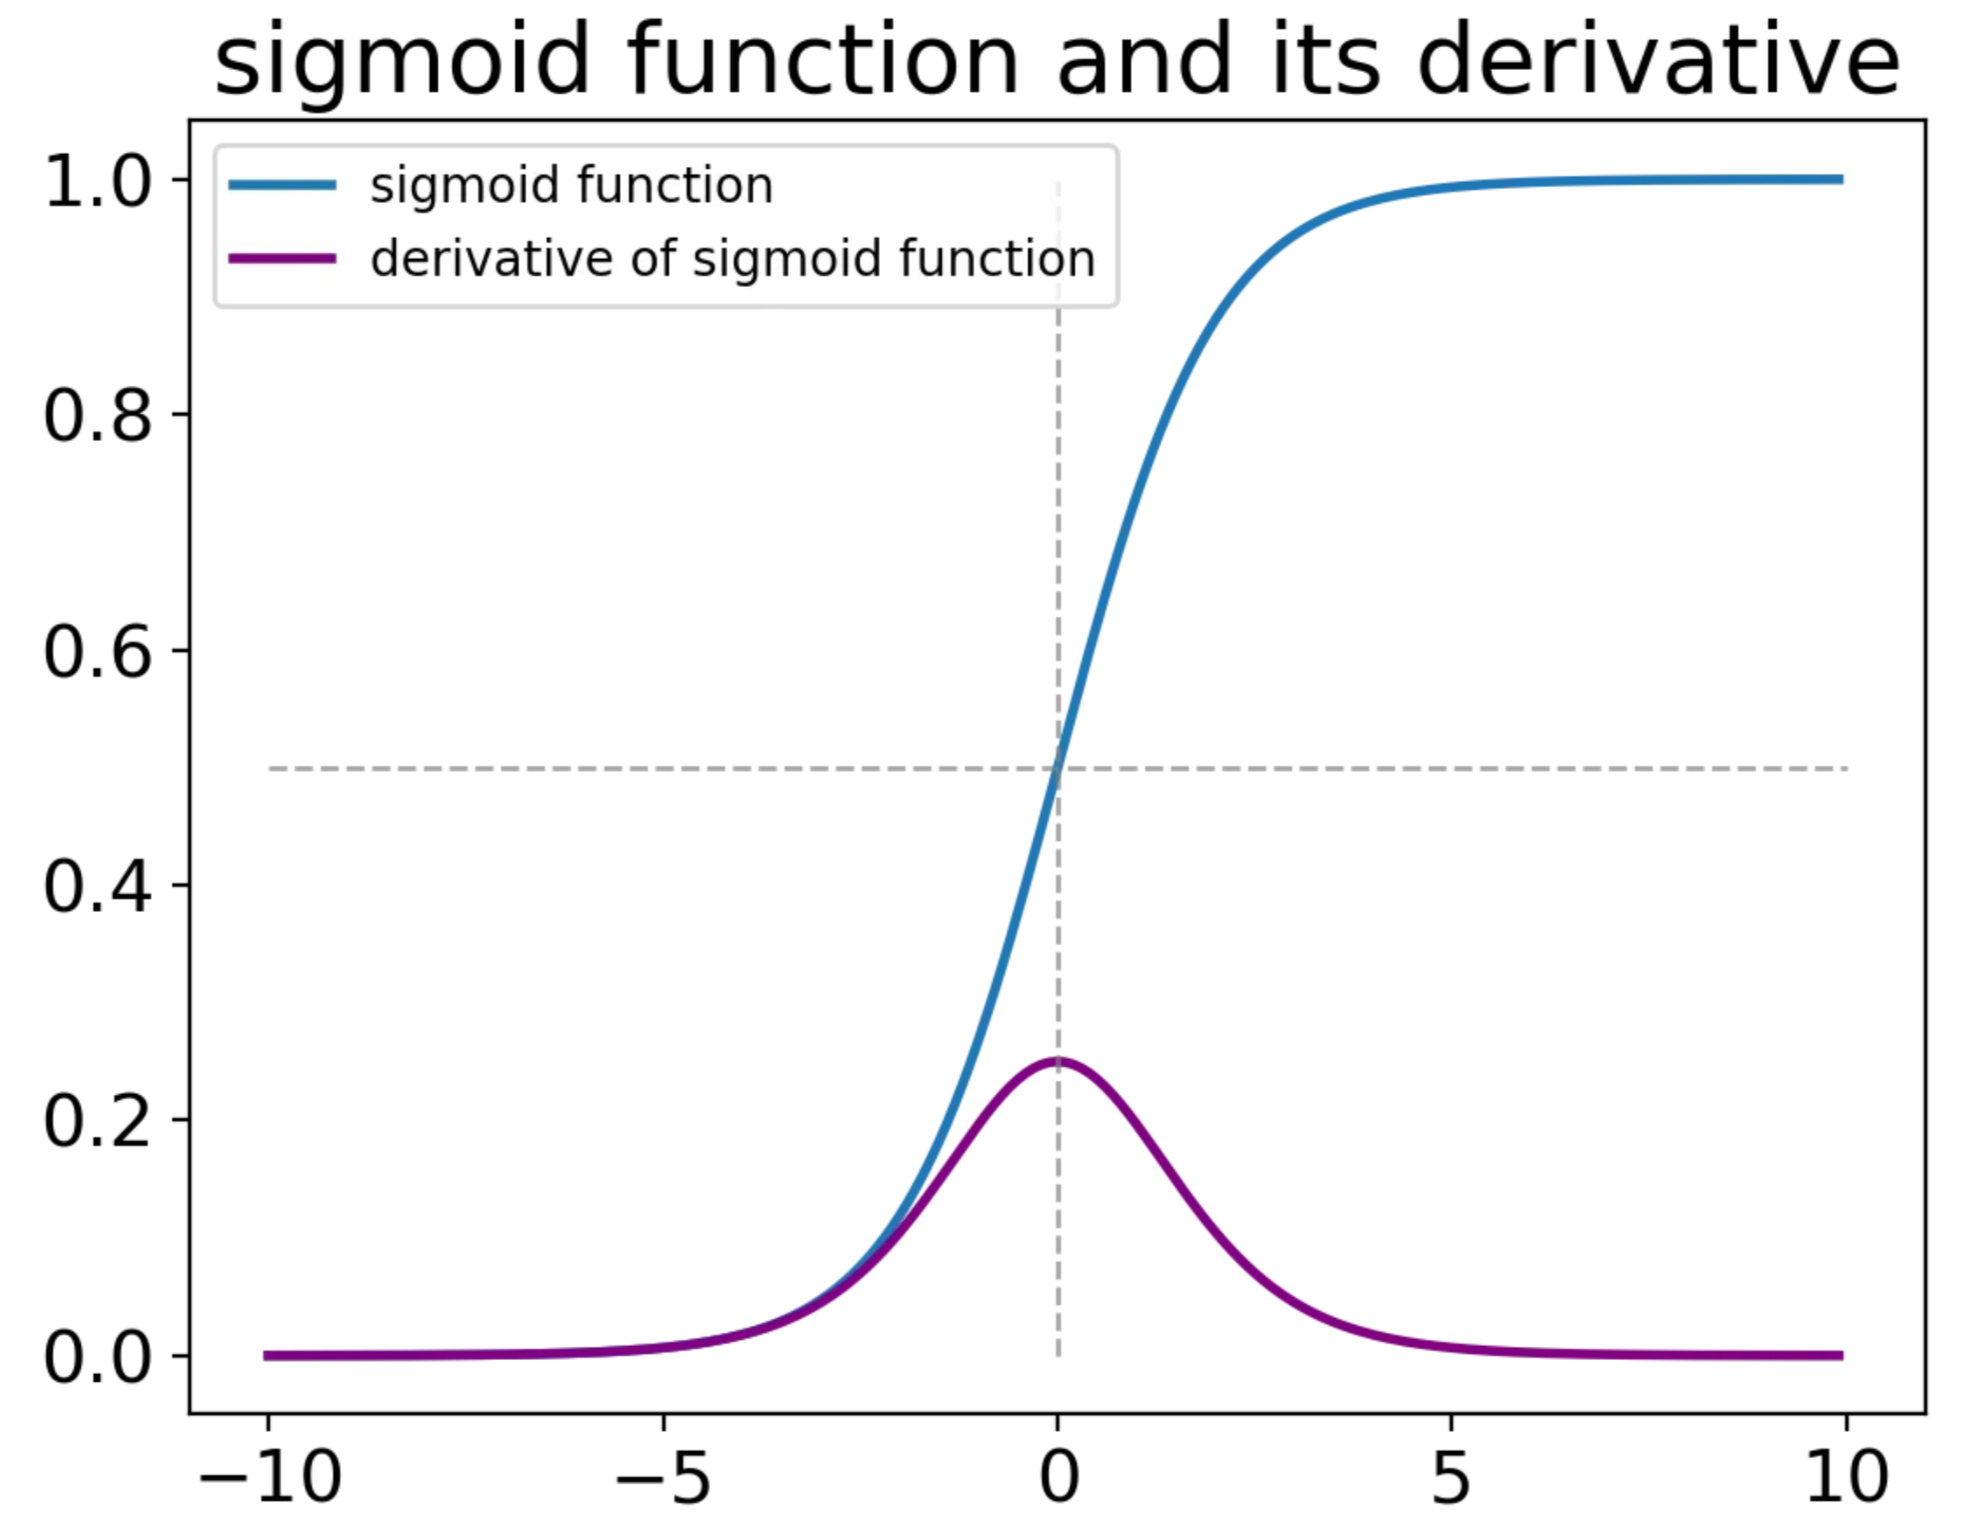
\includegraphics[width=0.3\linewidth]{images/sigmoid_derivative.png}
\end{figure}

\ideabox{
By passing our vector dot-product through the logistic mapping, we construct a hypothesis model that outputs a continuous probability score representing the confidence that a given instance belongs to the positive class.
}


\anondefinition{
Let $\mathbf{x} \in \mathbb{R}^{n+1}$ be an input feature vector and $\mathbf{w} \in \mathbb{R}^{n+1}$ be the parameter weight vector. The \defemph{Logistic Regression} hypothesis model $h_{\mathbf{w}}(\mathbf{x}) : \mathbb{R}^{n+1} \to (0, 1)$ is defined as:
\[
h_{\mathbf{w}}(\mathbf{x}) := \sigma(\mathbf{w}^T\mathbf{x}) = \frac{1}{1 + e^{-\mathbf{w}^T\mathbf{x}}}
\]
}{logistic_regression_hypothesis}

\commandnote{
This output explicitly models the conditional probability of the target label being positive given the features: $P(y=1 \mid \mathbf{x}, \mathbf{w})$.
}

\ideabox{
Because the output probability $h_{\mathbf{w}}(\mathbf{x})$ is a smooth, continuous curve between $0$ and $1$, we must establish a clear thresholding standard to make a final discrete binary prediction $\hat{y} \in \{0, 1\}$. By default, we assign an instance to the positive class if the model is more likely than not to belong there ($P \geq 0.5$).
}


To find the exact coordinates where the model switches its prediction from a negative class ($0$) to a positive class ($1$), we set the output probability to this $0.5$ threshold:
\[
h_{\mathbf{w}}(\mathbf{x}) = 0.5
\]
Substituting the definition of the logistic regression hypothesis:
\[
\frac{1}{1 + e^{-\mathbf{w}^T\mathbf{x}}} = \frac{1}{2}
\]
For these fractions to be equal, their denominators must be identical:
\[
1 + e^{-\mathbf{w}^T\mathbf{x}} = 2 \implies e^{-\mathbf{w}^T\mathbf{x}} = 1
\]
Taking the natural logarithm ($\ln$) of both sides isolates our input exponent:
\[
-\mathbf{w}^T\mathbf{x} = \ln(1)
\]
Since $\ln(1) = 0$, multiplying by $-1$ gives the threshold boundary equation:
\[
\mathbf{w}^T\mathbf{x} = 0
\]


\commandnote{
The algebraic condition $\mathbf{w}^T\mathbf{x} = 0$ defines the \defemph{decision boundary} of the logistic regression model. Because this dot product is a linear combination of the parameters and features, the boundary forms a flat, straight hyperplane embedded in the feature space $\mathbb{R}^n$.
}



\observationbox{
This derivation reveals our final classification rule explicitly:
\[
\hat{y} = \begin{cases} 
1 & \text{if } h_{\mathbf{w}}(\mathbf{x}) \geq 0.5 \iff \mathbf{w}^T\mathbf{x} \geq 0 \\
0 & \text{if } h_{\mathbf{w}}(\mathbf{x}) < 0.5 \iff \mathbf{w}^T\mathbf{x} < 0
\end{cases}
\]
}

\titledbox{Take-Home Message}{
Even though \linkterm{Logistic Regression}{logistic_regression_hypothesis} models continuous, curved probabilities using the non-linear sigmoid function ($\sigma$), the boundary it creates to separate classes is determined entirely by the linear equation $\mathbf{w}^T\mathbf{x} = 0$. Consequently, the boundary is always a flat straight line in 2D, a flat plane in 3D, or a flat hyperplane in higher dimensions. This proves mathematically that \linkterm{Logistic Regression}{logistic_regression_hypothesis} is strictly a \textbf{linear classifier} and can only separate data that is \linkterm{linearly separable}{decision_boundary}.
}

\ideabox{
We can use \linkterm{$\ell_2$ Loss}{l2_loss} and update the weights according to \linkterm{gradient descent}{gradient_descent_update}
}

Remember: The update rule for \linkterm{gradient descent}{gradient_descent_update}:
\[
\mathbf{w}^{(t+1)} := \mathbf{w}^{(t)} - \alpha \nabla L(\mathbf{w}^{(t)})
\]

Remember: \linkterm{$\ell_2$ Loss}{l2_loss}:
\[
\sum_{i=1}^{m} \big(y_i-h_{\mathbf{w}}(\mathbf{x})\big)^2.
\]

Let's derive \linkterm{stochastic gradient descent}{stochastic_gradient_descent} for \linkterm{logistic regression}{logistic_regression_hypothesis}
\[
h_{\mathbf{w}}(\mathbf{x}) := \sigma(\mathbf{w}^T\mathbf{x}) = \frac{1}{1 + e^{-\mathbf{w}^T\mathbf{x}}}
\]

Applying the chain rule to the single-instance squared loss function, the partial derivative with respect to a specific weight component $w_j$ is:
\[
\frac{\partial L}{\partial w_j} = \frac{\partial}{\partial w_j} \big(y_i - h_{\mathbf{w}}(\mathbf{x}^{(i)})\big)^2
\]

By the power rule, we bring down the exponent $2$ and multiply by the derivative of the inner function with respect to $w_j$:
\[
\frac{\partial L}{\partial w_j} = 2\big(y_i - h_{\mathbf{w}}(\mathbf{x}^{(i)})\big) \cdot \frac{\partial}{\partial w_j}\big(y_i - h_{\mathbf{w}}(\mathbf{x}^{(i)})\big)
\]

Since the true scalar label $y_i$ is a constant, its derivative vanishes ($=0$). This leaves the negative derivative of the hypothesis function:
\[
\frac{\partial L}{\partial w_j} = -2\big(y_i - h_{\mathbf{w}}(\mathbf{x}^{(i)})\big) \cdot \frac{\partial}{\partial w_j} h_{\mathbf{w}}(\mathbf{x}^{(i)})
\]

Substituting our logistic hypothesis model $h_{\mathbf{w}}(\mathbf{x}^{(i)}) = \sigma(\mathbf{w}^T\mathbf{x}^{(i)})$, we apply the chain rule again using the outer derivative of the sigmoid function, which we defined as $\sigma'(z)$:
\[
\frac{\partial L}{\partial w_j} = -2\big(y_i - h_{\mathbf{w}}(\mathbf{x}^{(i)})\big) \cdot \sigma'\big(\mathbf{w}^T\mathbf{x}^{(i)}\big) \cdot \frac{\partial}{\partial w_j}\big(\mathbf{w}^T\mathbf{x}^{(i)}\big)
\]

We now evaluate the two remaining inner parts of this product using our previous definitions:
\begin{itemize}
    \item The derivative of the sigmoid function satisfies $\sigma'(z) = \sigma(z)(1 - \sigma(z))$, meaning $\sigma'\big(\mathbf{w}^T\mathbf{x}^{(i)}\big) = h_{\mathbf{w}}(\mathbf{x}^{(i)})\big(1 - h_{\mathbf{w}}(\mathbf{x}^{(i)})\big)$.
    \item The derivative of the vector linear combination with respect to the coordinate weight parameter is $\frac{\partial}{\partial w_j}(\mathbf{w}^T\mathbf{x}^{(i)}) = x_j^{(i)}$.
\end{itemize}

Plugging both analytical terms back into our product yields the complete scalar gradient component for a single training instance:
\[
\frac{\partial L}{\partial w_j} = -2\big(y_i - h_{\mathbf{w}}(\mathbf{x}^{(i)})\big) \cdot h_{\mathbf{w}}(\mathbf{x}^{(i)})\big(1 - h_{\mathbf{w}}(\mathbf{x}^{(i)})\big) \cdot x_j^{(i)}
\]

\anondefinition{
By substituting this single coordinate derivative into the step update rule $w_j^{(t+1)} := w_j^{(t)} - \alpha \frac{\partial L}{\partial w_j}$, the double negatives cancel out. The final \defemph{logistic update rule} for a single parameter $w_j$ using a single training example under squared error loss is defined as:
\[
w_j^{(t+1)} := w_j^{(t)} + 2\alpha \big(y_i - h_{\mathbf{w}}(\mathbf{x}^{(i)})\big) \cdot h_{\mathbf{w}}(\mathbf{x}^{(i)})\big(1 - h_{\mathbf{w}}(\mathbf{x}^{(i)})\big) \cdot x_j^{(i)}
\]
}{logistic_update_rule_scalar}

\commandnote{
We sometimes multiply the \linkterm{loss function}{l2_loss} by $\frac{1}{2}$ before deriving so we can get rid of the constant factor $2$ in the final step adjustment:
\[
w_j^{(t+1)} := w_j^{(t)} + \alpha \big(y_i - h_{\mathbf{w}}(\mathbf{x}^{(i)})\big) \cdot h_{\mathbf{w}}(\mathbf{x}^{(i)})\big(1 - h_{\mathbf{w}}(\mathbf{x}^{(i)})\big) \cdot x_j^{(i)}
\]
}

